\section{Conclusion}

The intention of this work is to design the system to discover related articles in a large corpus automatically and evaluate the performance and usability thereof. We use \textit{Semantic Textual Similarity} (STS) methods as the main methods to quantify the relatedness degree between two articles. After the algorithms being to evaluate are selected, the different text fields in articles are also to evaluate. Therefore, the basic configuration of the system is the combination of an algorithm and a (preprocessed over n-gram) text field. We evaluate the effectiveness and efficiency of systems. Effectiveness which includes \textit{precision@2@3} and \textit{nDCG} is the measure of the quality of the outputted results of systems. Efficiency is the measure of the cost of resource (e.g. operational time) during running of systems to discover related articles. 

We setup the experiments to test the performance of static and dynamic systems using different combination of algorithms and text fields. ``Static'' means the corpus of articles is constant during the experiment. ``Dynamic'' means the corpus keeps increasing in running of systems, that is to say, once a target article have ``obtained'' related articles from systems, it is inserted immediately into the corpus as candidates of potential related article for future articles. The static experiment is used for comparing the performance of different STS methods in different text fields and the dynamic experiment focuses on the influence of the increasing corpus on the performance of systems. 

All STS methods are unsupervised and document-based, and hence the labels of training data and the information in meta-data are not utilized. In the viewpoint of the supervised approach, it is regarded as an application of learning to rank in the field of Information Retrieval. Therefore, the algorithms on learning to rank, such as logistic regression and ListNet, are set up on the base of the existed system to make full use of all kinds of data including meta-data and STS scores as features and improve the usability of the system.


\subsection{Answer of Research Question}

In this part, we summarize this work by way of answering the research questions which are raised in section \ref{sec:2.5}. 

\paragraph{Can Semantic Text Similarity including string-based and vector space models methods be used for finding related articles? How effective and efficient is the metrics of performance, such as precision and operational time?}

The former sub-question can be answered positively in section \ref{sec:5.3}. The system using \tfidf{} in text field \icontent{} over unigram has the best effectiveness with \textit{precision@2@3} of $45.07\%$ (see figure \ref{fig:precision_2_3}) and the acceptable efficiency (figure \ref{fig:build_time} and \ref{fig:predict_time}). Finding related articles for one target costs on average $340ms$\footnote{}, if the time of system building is taken into account.  

\paragraph{How do the methods work in the practical scenario that the corpus keeps increasing with time? How is the performance of the incremental system different from a constant system? }

From the results of the second experiment which are reported in section \ref{sec:5.4}, the STS methods work also well in the increasing candidate corpus. The effectiveness is better than the so-called ``out-of-date'' controlled system which is never updated in running and meanwhile worse than the other so-called ``coverall'' controlled system which is trained by the historical articles and future articles. In terms of efficiency, the time cost of system updating and predicting also increases linearly during corpus increasing. 


\paragraph{Is it useful to combine the STS methods? Does it yield to an improvement in performance?}

The question could be answered relative negatively due to the results in section \ref{sec:6.4}. The effectiveness of combinations (\#1, \#2, \#3 and \#4) of the STS methods is slightly higher than the system using the best single STS method. Therefore, combing the STS methods cannot lead to a significant improvement in performance. 

\paragraph{The above introduced methods are unsupervised and ignore other meta-data. Does it lead to an improvement with utilizing supervised or semi-supervised algorithms which are proposed in the field of learning to rank?}

The question can be answered positively also in section \ref{sec:6.4}. Logistic regression with the feature set of meta-data and the best STS methods over unigram yields to the highest improvement in effectiveness. The \textit{precision@2@3} of this system is $64.0\%$ and improved by $20.0$ percent compared with the baseline in the static experiment. On the other hand, the final system has the average \textit{precision@2@3} of $53.38\%$ and outperforms the baseline by $15.86$ percent. 

\subsection{Application in Reality}

The current system is able to discover two related articles for each target article with the precision of $53.38\%$ on average in the practical scenario. Due to the precision, the system cannot be used for replacing the manual assignment automatically. However, we can make use of the current system in the semi-automatic way to simplify the task of labeling by hand and improve the effectiveness and efficiency. Figure \ref{fig:top5} reports the moving average of the number of correct selections from the systems which find out $5$ related articles instead of $2$. In this system, $5$ articles are selected as related articles for each target and on average $2.18$ from the $5$ articles are judged correctly. Moreover, more than $2$ articles are judged correctly in the most predictions. From this results, the entire process is accomplished by cooperation between the system and the author. That is to say, 5 articles are found out by the system as potential related articles and then the author selects two articles from the picked candidates as the final related articles. 

\clearpage

\begin{figure}[!htb]
    \centering
    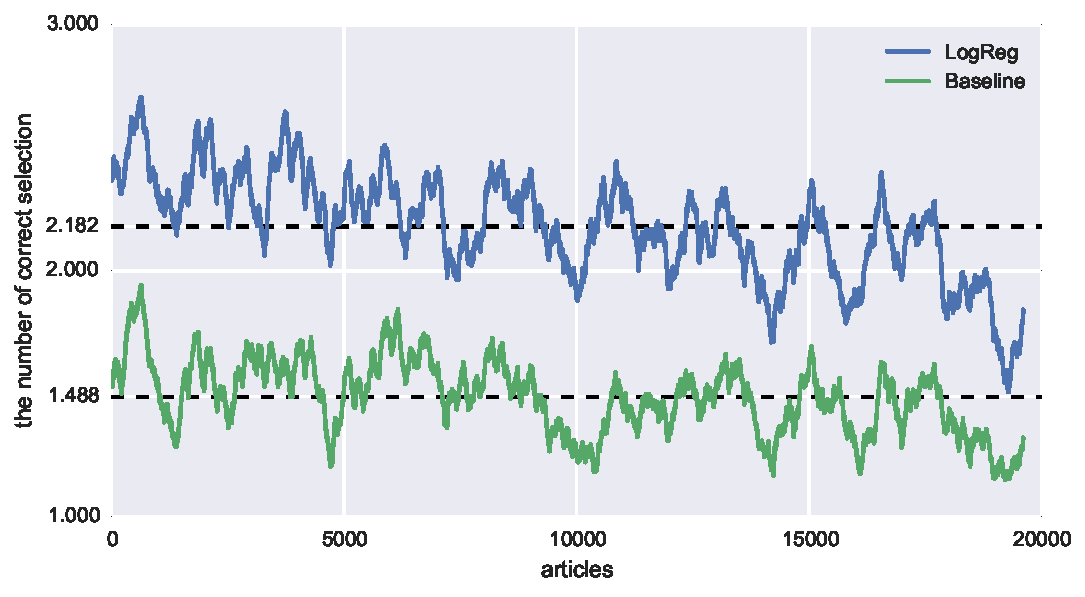
\includegraphics[width=\textwidth]{fig/precision_inc_supervised_5}
    \caption[The moving average of the number of correct selection of related articles by the system which selects $5$ related articles]{The moving average of the number of correct selections of related articles by the system which selects $5$ related articles instead of $2$ articles}
    \label{fig:top5}
\end{figure}

\subsection{Future Work}

The factors affecting the relatedness degree between two articles are not completely clear. Therefore, it must lead to bias that \textit{Semantic Textual Similarity} is used as the single semantic measure to quantify the relatedness degree. In other words, the current system is just able to discover articles which are semantic similar to the target as related articles. Nevertheless, two articles are related to each other because they are not only similar in semantics but also have other relationships, like causal relationship. Eliminating or reducing bias becomes the main issue in the future work. The next step of the research can be divided into two directions. One direction is to find other measures to describe particular semantic relationships and add them into the feature set. The other direction is to make a study of the general approach to depict the characteristics of any relationship between two articles. Furthermore, some latent but useful features may improve the usability of the system, and we can generate more features from the information of articles besides meta-data. 


